\documentclass[aspectratio=169,10pt]{beamer}
\usetheme{default}
\usecolortheme{dove}
\setbeamertemplate{navigation symbols}{}
\setbeamertemplate{footline}[frame number]
\usepackage[T1]{fontenc}
\usepackage{booktabs,siunitx,graphicx}
\graphicspath{{../results/paper_figures/}}
\makeatletter\newcommand{\tabinput}[1]{\@@input #1.tex }\makeatother
% Auto-generated by scripts/study/analyze.py -- do not edit.
\newcommand{\BanditMinusCspf}{50.8}
\newcommand{\BanditMinusCspfHi}{53.7}
\newcommand{\BanditMinusCspfLo}{47.1}
\newcommand{\BanditMinusGreedy}{21.2}
\newcommand{\BanditMinusGreedyHi}{24.1}
\newcommand{\BanditMinusGreedyLo}{17.6}
\newcommand{\BanditMinusMilp}{5.2}
\newcommand{\BanditMinusMilpHi}{8.1}
\newcommand{\BanditMinusMilpLo}{1.3}
\newcommand{\BanditMinusNoop}{120.7}
\newcommand{\BanditMinusNoopHi}{123.6}
\newcommand{\BanditMinusNoopLo}{117.0}
\newcommand{\BanditMinusOracleOne}{-29.2}
\newcommand{\BanditMinusOracleOneHi}{-23.7}
\newcommand{\BanditMinusOracleOneLo}{-36.1}
\newcommand{\BanditMinusRandom}{132.7}
\newcommand{\BanditMinusRandomHi}{136.1}
\newcommand{\BanditMinusRandomLo}{128.7}
\newcommand{\BanditMinusStatic}{121.7}
\newcommand{\BanditMinusStaticHi}{124.6}
\newcommand{\BanditMinusStaticLo}{118.0}
\newcommand{\BaselineReproCells}{21}
\newcommand{\BaselineReproMaxDiff}{3\cdot10^{-14}}
\newcommand{\Gap}{30.6}
\newcommand{\GapDeceptive}{14.6}
\newcommand{\GapDoublefailure}{-2.3}
\newcommand{\GapDz}{0.76}
\newcommand{\GapEveningpeak}{37.6}
\newcommand{\GapFinal}{39.1}
\newcommand{\GapFinalHi}{67.5}
\newcommand{\GapFinalLo}{3.5}
\newcommand{\GapFinalRootsPositive}{3}
\newcommand{\GapFlashcrowd}{23.6}
\newcommand{\GapFullday}{103.1}
\newcommand{\GapHi}{50.6}
\newcommand{\GapLinkfailure}{16.9}
\newcommand{\GapLo}{9.1}
\newcommand{\GapOverload}{20.3}
\newcommand{\GapRoots}{3}
\newcommand{\GapRootsPositive}{3}
\newcommand{\GapTHi}{82.8}
\newcommand{\GapTLo}{-21.7}
\newcommand{\GapWinRate}{86}
\newcommand{\HistBandit}{18.2}
\newcommand{\HistBanditRootA}{16.1}
\newcommand{\HistBanditRootB}{20.5}
\newcommand{\HistBanditRootC}{18.0}
\newcommand{\HistDeceptive}{-1.1}
\newcommand{\HistGap}{9.2}
\newcommand{\HistGapTHi}{17.3}
\newcommand{\HistGapTLo}{1.1}
\newcommand{\HistPPO}{9.0}
\newcommand{\HistPPORootA}{6.6}
\newcommand{\HistPPORootB}{8.3}
\newcommand{\HistPPORootC}{12.2}
\newcommand{\NDemands}{17}
\newcommand{\NDirLinks}{64}
\newcommand{\NLinks}{32}
\newcommand{\NRouters}{18}
\newcommand{\PPOMinusCspf}{19.2}
\newcommand{\PPOMinusCspfHi}{42.2}
\newcommand{\PPOMinusCspfLo}{3.4}
\newcommand{\PPOMinusGreedy}{-10.4}
\newcommand{\PPOMinusGreedyHi}{12.7}
\newcommand{\PPOMinusGreedyLo}{-26.2}
\newcommand{\PPOMinusMilp}{-34.1}
\newcommand{\PPOMinusMilpHi}{-7.8}
\newcommand{\PPOMinusMilpLo}{-55.7}
\newcommand{\PPOMinusNoop}{89.1}
\newcommand{\PPOMinusNoopHi}{112.1}
\newcommand{\PPOMinusNoopLo}{73.3}
\newcommand{\PPOMinusOracleOne}{-133.4}
\newcommand{\PPOMinusOracleOneHi}{-71.3}
\newcommand{\PPOMinusOracleOneLo}{-188.5}
\newcommand{\PPOMinusRandom}{101.1}
\newcommand{\PPOMinusRandomHi}{123.7}
\newcommand{\PPOMinusRandomLo}{85.5}
\newcommand{\PPOMinusStatic}{90.1}
\newcommand{\PPOMinusStaticHi}{113.1}
\newcommand{\PPOMinusStaticLo}{74.3}
\newcommand{\PeakOfferedGbps}{2.49}
\newcommand{\ReproBandit}{18.0}
\newcommand{\ReproBanditRootA}{14.7}
\newcommand{\ReproBanditRootB}{17.2}
\newcommand{\ReproBanditRootC}{22.2}
\newcommand{\ReproDeceptive}{14.7}
\newcommand{\ReproDeceptiveHi}{18.9}
\newcommand{\ReproDeceptiveLo}{10.6}
\newcommand{\ReproGap}{30.1}
\newcommand{\ReproGapHi}{50.8}
\newcommand{\ReproGapLo}{4.4}
\newcommand{\ReproMaxShiftBandit}{4}
\newcommand{\ReproMaxShiftPPO}{41}
\newcommand{\ReproPPO}{-12.0}
\newcommand{\ReproPPONeverPositive}{2}
\newcommand{\ReproPPORootA}{-20.1}
\newcommand{\ReproPPORootB}{13.0}
\newcommand{\ReproPPORootC}{-29.0}
\newcommand{\ReproRoots}{3}
\newcommand{\ReproRootsPositive}{3}
\newcommand{\SeqLiveAgreeH1}{100}
\newcommand{\SeqLiveAgreeH12}{46}
\newcommand{\SeqLiveAgreeH24}{34}
\newcommand{\SeqLiveAgreeH3}{73}
\newcommand{\SeqLiveAgreeH6}{56}
\newcommand{\SeqLiveCapturedH1}{100}
\newcommand{\SeqLiveCapturedH12}{59}
\newcommand{\SeqLiveCapturedH24}{52}
\newcommand{\SeqLiveCapturedH3}{78}
\newcommand{\SeqLiveCapturedH6}{61}
\newcommand{\SeqLiveSacrificeH1}{0}
\newcommand{\SeqLiveSacrificeH12}{45}
\newcommand{\SeqLiveSacrificeH24}{59}
\newcommand{\SeqLiveSacrificeH3}{19}
\newcommand{\SeqLiveSacrificeH6}{35}
\newcommand{\SeqLiveStates}{289}
\newcommand{\TestBandit}{25.2}
\newcommand{\TestBanditDecisionMs}{0.37}
\newcommand{\TestBanditDelivered}{95.31}
\newcommand{\TestBanditHi}{28.1}
\newcommand{\TestBanditLo}{21.5}
\newcommand{\TestBanditReroutes}{2.30}
\newcommand{\TestBanditRoots}{5}
\newcommand{\TestBanditSla}{164}
\newcommand{\TestCspf}{-25.6}
\newcommand{\TestCspfDecisionMs}{0.06}
\newcommand{\TestCspfDelivered}{93.64}
\newcommand{\TestCspfHi}{-23.2}
\newcommand{\TestCspfLo}{-28.0}
\newcommand{\TestCspfReroutes}{0.61}
\newcommand{\TestCspfRoots}{0}
\newcommand{\TestCspfSla}{243}
\newcommand{\TestGreedy}{4.0}
\newcommand{\TestGreedyDecisionMs}{0.06}
\newcommand{\TestGreedyDelivered}{94.85}
\newcommand{\TestGreedyHi}{6.3}
\newcommand{\TestGreedyLo}{1.7}
\newcommand{\TestGreedyReroutes}{4.60}
\newcommand{\TestGreedyRoots}{0}
\newcommand{\TestGreedySla}{187}
\newcommand{\TestMilp}{80.8}
\newcommand{\TestMilpDecisionMs}{637.23}
\newcommand{\TestMilpDelivered}{97.62}
\newcommand{\TestMilpHi}{83.4}
\newcommand{\TestMilpLo}{78.2}
\newcommand{\TestMilpReroutes}{5.68}
\newcommand{\TestMilpRoots}{0}
\newcommand{\TestMilpSla}{136}
\newcommand{\TestNoop}{-95.5}
\newcommand{\TestNoopDecisionMs}{0.00}
\newcommand{\TestNoopDelivered}{90.58}
\newcommand{\TestNoopHi}{-92.9}
\newcommand{\TestNoopLo}{-98.0}
\newcommand{\TestNoopReroutes}{0.00}
\newcommand{\TestNoopRoots}{0}
\newcommand{\TestNoopSla}{352}
\newcommand{\TestOracleOne}{372.3}
\newcommand{\TestOracleOneDecisionMs}{1649.99}
\newcommand{\TestOracleOneDelivered}{99.19}
\newcommand{\TestOracleOneHi}{380.8}
\newcommand{\TestOracleOneLo}{364.2}
\newcommand{\TestOracleOneReroutes}{1.07}
\newcommand{\TestOracleOneRoots}{0}
\newcommand{\TestOracleOneSla}{113}
\newcommand{\TestPPO}{-6.4}
\newcommand{\TestPPODecisionMs}{1.12}
\newcommand{\TestPPODelivered}{94.97}
\newcommand{\TestPPOHi}{16.6}
\newcommand{\TestPPOLo}{-22.2}
\newcommand{\TestPPOReroutes}{8.94}
\newcommand{\TestPPORoots}{3}
\newcommand{\TestPPOSla}{182}
\newcommand{\TestRandom}{-107.5}
\newcommand{\TestRandomDecisionMs}{0.02}
\newcommand{\TestRandomDelivered}{89.44}
\newcommand{\TestRandomHi}{-103.6}
\newcommand{\TestRandomLo}{-111.3}
\newcommand{\TestRandomReroutes}{11.66}
\newcommand{\TestRandomRoots}{0}
\newcommand{\TestRandomSla}{401}
\newcommand{\TestStatic}{-96.5}
\newcommand{\TestStaticDecisionMs}{0.01}
\newcommand{\TestStaticDelivered}{90.40}
\newcommand{\TestStaticHi}{-94.0}
\newcommand{\TestStaticLo}{-98.9}
\newcommand{\TestStaticReroutes}{0.37}
\newcommand{\TestStaticRoots}{0}
\newcommand{\TestStaticSla}{346}
\newcommand{\TotalCapacityGbps}{45.0}
\newcommand{\TpsBandit}{147}
\newcommand{\TpsPPO}{140}
\newcommand{\WallBandit}{45}
\newcommand{\WallPPO}{48}

\newcommand{\hl}[1]{\textcolor[HTML]{2A78D6}{\textbf{#1}}}

\title{Persistent state is not enough}
\subtitle{A controlled study of planning horizons in incremental MPLS traffic engineering}
\author{Uğur Efe Yiğit}
\date{}

\begin{document}

\begin{frame}
\titlepage
\end{frame}

\begin{frame}{1. Problem: incremental MPLS traffic engineering}
\begin{columns}
\column{0.52\textwidth}
\begin{itemize}
\item 18 routers, 64 directed links, 17 demands with SLAs, 4 candidate LSPs each
\item every 5 min: move \emph{one} demand to another candidate, or do nothing
\item moves cost reconfiguration effort; 3-interval hold-down after a move
\item action mask: failed links, hold-down, protected-class capacity
\item reward: delivery, disconnection, SLA severity, utilization, overload, minus move costs
\end{itemize}
\column{0.46\textwidth}
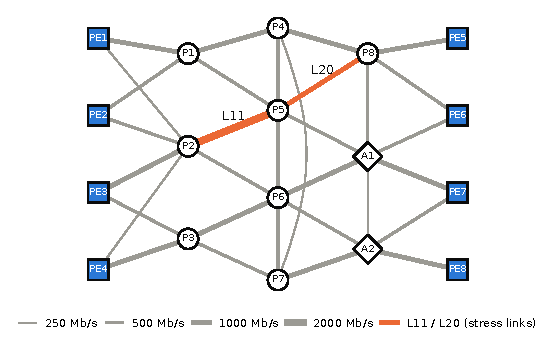
\includegraphics[width=\textwidth]{fig_topology}
\end{columns}
\end{frame}

\begin{frame}{2. Why RL --- and why sequentiality should not be assumed}
\begin{itemize}
\item routes \hl{persist}, moves lock a demand, protected-class legality couples demands
  $\Rightarrow$ formally an MDP
\item but a move carries traffic \emph{in the interval it is made}, traffic is exogenous
\item recent TE systems treat TE as one-shot (Teal, DOTE) --- in a setting \emph{without} persistent state
\item \textbf{Question:} here, does a learner that plans ($\gamma=0.995$) beat one that only
  predicts the immediate reward ($\gamma=0$)? Why?
\end{itemize}
\end{frame}

\begin{frame}{3. The surprising observation, reproduced}
\begin{itemize}
\item closed predecessor study: bandit \HistBandit{} vs PPO \HistPPO{} (holdout return, 3 roots)
\item retrained everything on different hardware, byte-identical training traffic:
  \begin{itemize}
  \item baselines: \hl{exact} ($\BaselineReproMaxDiff$)
  \item bandit: \hl{reproduces} (\ReproBandit)
  \item PPO: \hl{does not} (\ReproPPO); per-root shifts up to \ReproMaxShiftPPO{} points
  \item ``PPO wins the deceptive scenario'': does not reproduce
  \end{itemize}
\end{itemize}
\vspace{1ex}
\small
\begin{tabular}{@{}lrcrr@{}}
\toprule
Learner & Root & Selected (h./r.) & Hist. & Repr. \\
\midrule
\tabinput{../paper/tables/reproduction_per_root}
\bottomrule
\end{tabular}
\end{frame}

\begin{frame}{4. Methodology}
\begin{itemize}
\item same observation (604), mask, budget (400k transitions), paired traffic
\item select on validation seeds, report on 140 disjoint test episodes; 5 training roots
\item two-stage bootstrap CIs over roots and episodes
\item references: static, greedy, CSPF, \hl{MILP-track} (per-interval min-max-util),
  clairvoyant Oracle-$H$
\item controls: PPO $\gamma\in\{0,0.9,0.995\}$; masked Q-learner $\gamma\in\{0,0.5,0.9,0.99\}$
  ($\gamma=0$ = bandit, bit-identical); PPO tuning; delayed-effect variant; time-of-day observation
\end{itemize}
\end{frame}

\begin{frame}{5. Result: bandit $>$ PPO; a tuned per-interval optimizer beats both}
\begin{columns}
\column{0.62\textwidth}
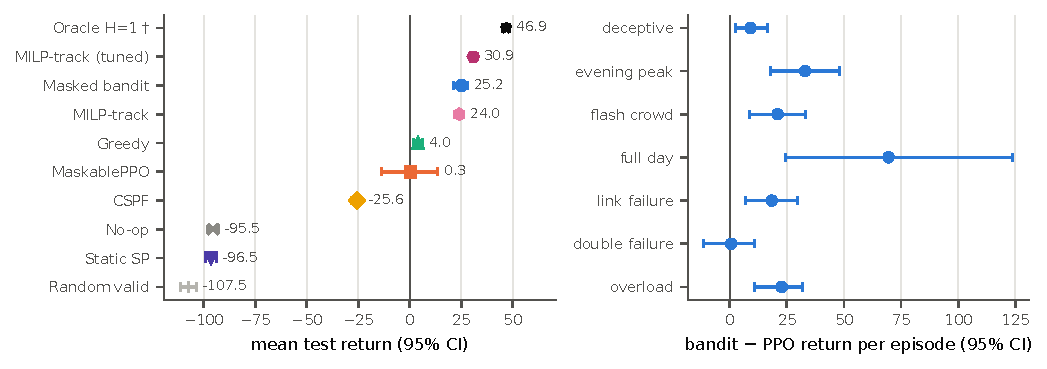
\includegraphics[width=\textwidth]{fig_main}
\column{0.36\textwidth}
\small
\begin{itemize}
\item bandit $-$ PPO $=$ \hl{\Gap}, $t$-interval over roots [\GapTLo, \GapTHi], positive on \GapRootsPositive/\GapRoots{} roots
\item bandit $-$ MILP-track (untuned) $=$ \BanditMinusMilp{} [\BanditMinusMilpTLo, \BanditMinusMilpTHi]
\item MILP-track tuned on validation: \hl{\TestMilpTuned}, ahead of the bandit on every root
\item reroutes/h: bandit \TestBanditReroutes, MILP \TestMilpReroutes, PPO \TestPPOReroutes
\end{itemize}
\end{columns}
\end{frame}

\begin{frame}{6. Mechanism: PPO flaps at hold-down expiry}
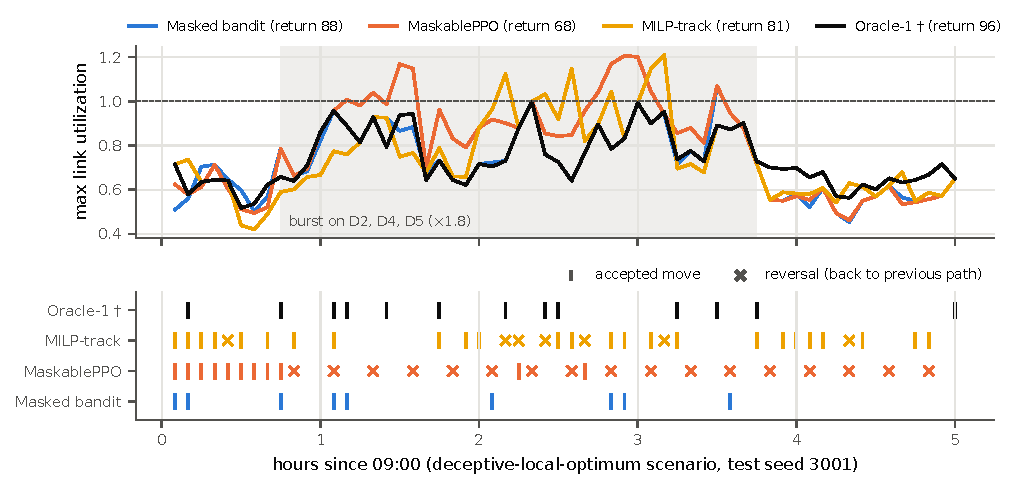
\includegraphics[width=\textwidth]{fig_case}
\small Utility: bandit \UtilBandit, PPO \UtilPPO; move costs: bandit \CostBandit, PPO \CostPPO
\end{frame}

\begin{frame}{7. Attribution: the horizon, not the algorithm (so far)}
\begin{columns}
\column{0.5\textwidth}
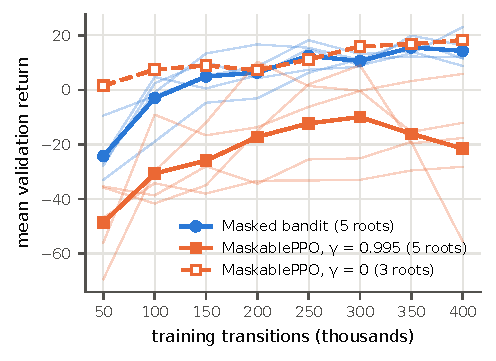
\includegraphics[width=\textwidth]{fig_learning_curves}
\column{0.48\textwidth}
\begin{itemize}
\item PPO with $\gamma=0$: \hl{\HPPOZero} vs bandit \HQZero{} on the same roots
\item difference \HPPOZeroVs{} [\HPPOZeroVsLo, \HPPOZeroVsHi]
\item flapping disappears
\item return falls with $\gamma$ in both families (PPO $\gamma=0.9$: \HPPOPointNine; Q $\gamma=0.99$: \HQPointNineNine)
\item tuned PPO (best of 8 on one root) below the bandit on all \RQThreeTunedVsBanditRoots{} fresh roots
\item hypothesis: small one-off costs drowned by long-horizon advantage noise
\end{itemize}
\end{columns}
\end{frame}

\begin{frame}{8. How sequential is the problem?}
\begin{columns}
\column{0.58\textwidth}
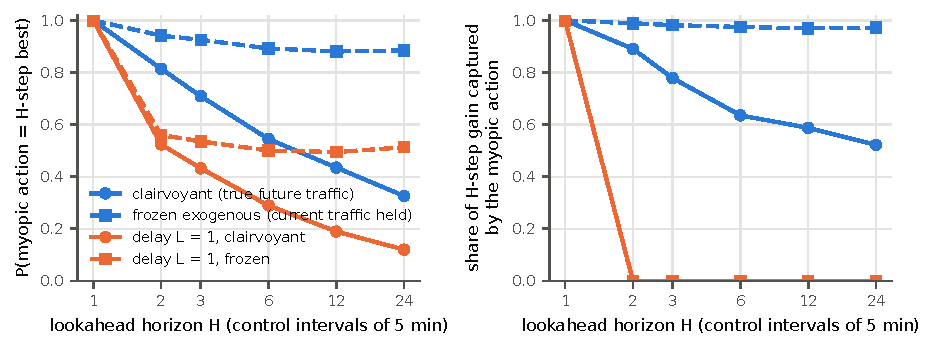
\includegraphics[width=\textwidth]{fig_seqdiag}
\column{0.4\textwidth}
\small
\begin{itemize}
\item re-planning with perfect foresight: 3-step lookahead adds only \OracleThreeMinusOne{}
\item open loop, true future: myopic $=$ 24-step best in \SeqLiveAgreeHTwentyFour\,\% of states
\item traffic frozen: \hl{\SeqFrozenAgreeHTwentyFour\,\%}
\item open-loop non-myopic value $\approx$ anticipating exogenous change, not provided by the observation
\item \hl{but}: with a greedy controller reacting after the first move, agreement falls to \SeqContLiveAgreeHTwentyFour\,\% (frozen \SeqContFrozenAgreeHTwentyFour\,\%) --- first moves shape later value; the learners did not exploit it
\end{itemize}
\end{columns}
\end{frame}

\begin{frame}{9. When does the myopic learner fail? Delay the effect of a move}
\begin{columns}
\column{0.55\textwidth}
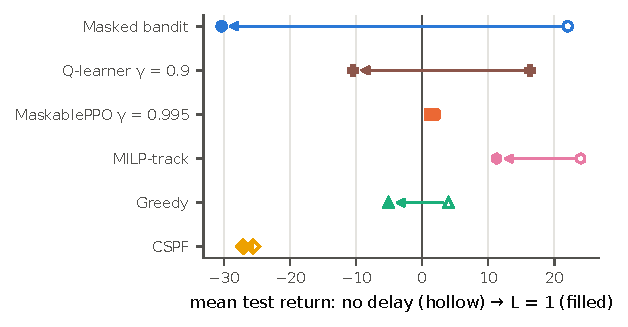
\includegraphics[width=\textwidth]{fig_delay}
\column{0.43\textwidth}
\small
\begin{itemize}
\item move requested at $t$, active from $t+1$: the immediate reward contains only its cost
\item bandit: \DelayBanditLZero{} $\to$ \hl{\DelayBandit}
\item PPO: \DelayPPOLZero{} $\to$ \DelayPPO{} (mean; per-root shifts in both directions)
\item PPO $-$ bandit under delay: \hl{\DelayPPOVs} (mean), ahead on
  \DelayPPORootsBetter/\DelayPPORoots{} roots
\item MILP-track: \DelayRefmilptrackLZero{} $\to$ \DelayRefmilptrack{} --- still ahead of every learner
\item shows: decision-time regression fails; not that long-horizon RL is needed
\item the rollout diagnostic flags it without training: myopic choice captures \SeqDelayFrozenCapturedHTwentyFour\,\% of the 24-step gain (\SeqFrozenCapturedHTwentyFour\,\% at $L=0$)
\end{itemize}
\end{columns}
\end{frame}

\begin{frame}{10. Clairvoyance: how much is lookahead worth?}
\begin{itemize}
\item Oracle-$H$: enumerates every legal move with the true future, no-op continuation
\item Oracle-1 \LadderOraclehOne, Oracle-3 \LadderOraclehThree, Oracle-6 \LadderOraclehSix{} (5 test seeds)
\item Oracle-3 $-$ Oracle-1 $=$ \OracleThreeMinusOne{} [\OracleThreeMinusOneLo, \OracleThreeMinusOneHi];
  Oracle-6 $-$ Oracle-1 $=$ \OracleSixMinusOne{} [\OracleSixMinusOneLo, \OracleSixMinusOneHi]
\item bandit $-$ Oracle-1 $=$ \BanditMinusOracleOne{}: \hl{knowing the next interval} is worth far
  more than planning beyond it
\end{itemize}
\end{frame}

\begin{frame}{11. Limitations}
\begin{itemize}
\item flow-level model, exogenous inelastic traffic, instantaneous control plane
\item one topology, scripted scenarios, one reward; 5 (main) / 2--3 (ablation) roots
\item single-move-per-interval formulation is a design choice
\end{itemize}
\end{frame}

\begin{frame}{12. Take-aways and future work}
\begin{itemize}
\item measure the value of lookahead before choosing a sequential learner: the rollout diagnostic separated the base and the delayed regime without training
\item learner noise within a root is large (\NoiseBanditSpread{} points): small effects need many roots
\item a tuned per-interval optimizer is the baseline to beat; a myopic learner is next
\item long horizons can hurt by hiding small immediate costs
\item future: delayed actuation and elastic traffic; packet-level validation; GNN policies;
  larger topologies; real traffic matrices
\end{itemize}
\end{frame}

\end{document}
